 \documentclass[a4paper,12pt]{article}
\usepackage[utf8]{inputenc}
\usepackage{csquotes}
\usepackage[ngerman]{babel}
\usepackage{biblatex}
\usepackage{float}
\usepackage{graphicx}
\usepackage{epstopdf}
\usepackage{subfigure}
\usepackage{graphvizzz}
\usepackage{array}
\usepackage[table]{xcolor}
\usepackage{booktabs}
\usepackage{listings}
\usepackage{multirow}
\usepackage[format=plain,labelfont=bf,up,justification=centering]{caption}
\setcounter{secnumdepth}{-1} 
\usepackage{hyperref}
\usepackage{nameref}
%\usepackage{minted}
%\usemintedstyle{friendly}
\lstdefinelanguage{JavaScript}{
  keywords={typeof, new, true, false, catch, function, return, null, catch, switch, var, if, in, while, do, else, case, break},
  keywordstyle=\color{blue}\bfseries,
  ndkeywords={class, export, boolean, throw, implements, import, this},
  ndkeywordstyle=\color{darkgray}\bfseries,
  identifierstyle=\color{black},
  sensitive=false,
  comment=[l]{//},
  morecomment=[s]{/*}{*/},
  commentstyle=\color{purple}\ttfamily,
  stringstyle=\color{red}\ttfamily,
  morestring=[b]',
  morestring=[b]"
}
\lstset{
   language=JavaScript,
   backgroundcolor=\color{lightgray},
   extendedchars=true,
   basicstyle=\footnotesize\ttfamily,
   showstringspaces=false,
   showspaces=false,
   numbers=left,
   numberstyle=\footnotesize,
   numbersep=9pt,
   tabsize=2,
   breaklines=true,
   showtabs=false,
   captionpos=b
}

\bibliography{documentation}
\title{Gesture Remote \\ VLC Remote Control für die Android-Plattform}
\author{Andreas Feldmann \\ Willi Schönborn}
\date{\today}
\begin{document}

\begin{figure}[H]
\centering

\includegraphics[width=0.5\textwidth]{beuth.eps}
\maketitle
\end{figure}
\newpage
\tableofcontents
\newpage
\section{Projektidee}
Zur Zeit steigt die Nachfrage nach gut bedienbaren Streamingsystemen für den Heimbereich immer weiter an. Dabei wird nicht mehr nur auf die Installation und Wartbarkeit wert gelegt, sondern auch auf die Bedienbarkeit. Und doch können fest installierte Geräte mit Streamingsoftware meist nur über die eingesetzten Peripheriegeräte gesteuert werden. \\
Da sich in den meisten dieser Haushalte auch ein mobiles Endgerät befindet, wäre eine Steuerung der Software über diese Technologie von Vorteil. Dabei spielt vor allem die Art der Steuerung eine wichtige Rolle. Der Benutzer soll nicht nur eine Oberfläche mit entsprechenden Schaltflächen vorfinden, sondern prägnante Gesten, die sich wie bei älteren Geräten vor findbar, für eine simple Benutzung sorgen. Damit würde, wie bei klassischen TV-Geräten, eine Fernbedienung geschaffen die sich an den einprägsamen Bewegungen (in diesem Fall Gesten) orientiert. \\
Dieses Projekt soll sich mit der Umsetzung einer solchen Remotesteuerung von einem mobilen Endgerät aus, zur Streamingsoftware beschäftigen.

Es gibt frei verfügbare Apps mit ähnlichen Ansätzen. Am interessantesten ist wohl die \textit{Android VLC Remote} App \cite{android-vlc-remote}. Das größte Manko an Apps dieser Art ist, unserer Meinung nach, dass die Möglichkeiten des Smartphones nicht voll ausgereizt werden und damit die Möglichkeiten für eine größere Nutzerzufriedenheit nicht in dem Maße ausgeschöpft werden wie sie könnten.

\newpage
\section{Konzept}

\subsection{Gesten}
Alle letztendlich unterstützten Gesten sollen den folgenden Kriterien genügen. Durch die Einhaltung dieser Kriterien versprechen wir uns eine kurze Lernphase und damit extrem kleine Einstiegshürde für Nutzer der App.

\begin{itemize}
	\item \textbf{Erwartungskonform} \\
		Gesten wie Flick, Tap und Scale sind durch bestehende Apps bei vielen Nutzern bereits mental mit entsprechenden Funktionen verknüpft. Diese Erwartungshaltung sollte, sofern möglich, erfüllt werden.
	\item \textbf{Innovativ} \\
		Falls es für bestimmte Funktionen noch keinen De facto-Standard gibt was eine Gestensteuerung betrifft, so sollen neue Gesten gefunden werden, die ggf. so noch nicht genutzt wurden. Wichtig dabei ist jedoch der nächste Punkt.
	\item \textbf{Intuitiv und nachvollziehbar} \\
		Bei neuartigen, ungewohnten oder seltenen Gesten sollte eine Funktion angestoßen werden, die sinnvoll zur entsprechenden Geste passt. Hier sind ggf. kleine A/B-Tests oder eng gefasste Spartakusgruppe-Interviews sinnvoll.
\end{itemize}

Abbildung \ref{fig:gestures} zeigt einige Gesten die ad hoc in Frage kommen sowie mögliche Funktionen, mit denen sie verknüpft werden könnten.

\begin{figure}[H]
\centering
\subfigure[Play/Pause]{
    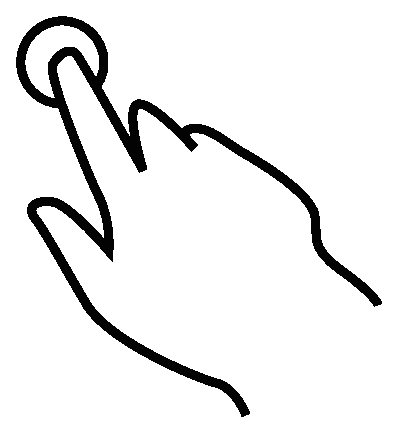
\includegraphics[width=0.2\textwidth]{one_finger_tap_gestureworks.eps}
}
\subfigure[Nächster Titel]{
    \reflectbox{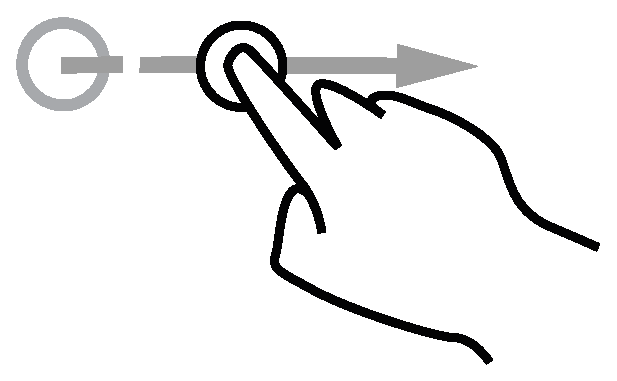
\includegraphics[width=0.35\textwidth]{one_finger_flick_gestureworks.eps}}
}
\subfigure[Vorheriger Titel]{
    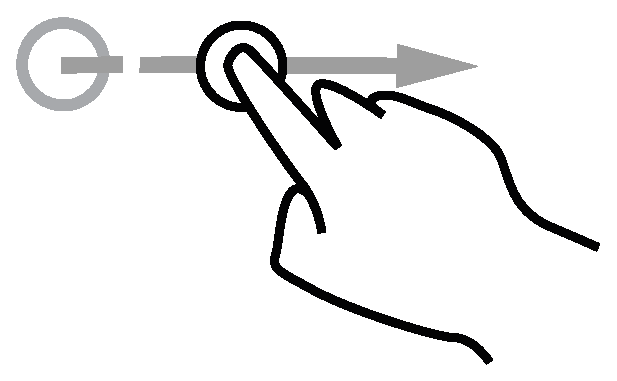
\includegraphics[width=0.35\textwidth]{one_finger_flick_gestureworks.eps}
}
\subfigure[Volume/Seek]{
    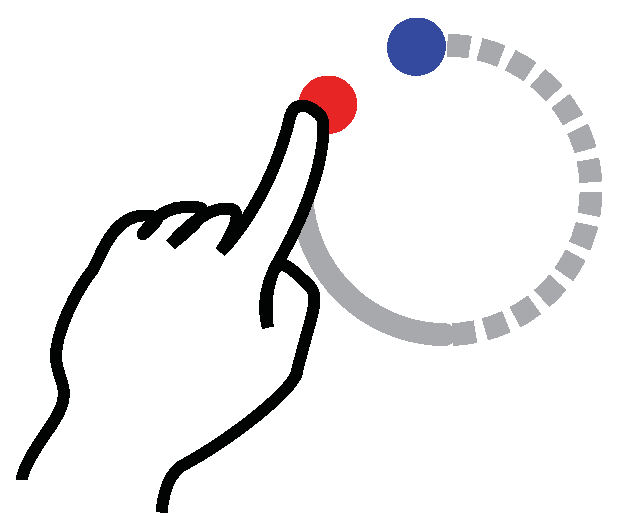
\includegraphics[width=0.3\textwidth]{stroke_shape_circle_gestureworks.eps}
    \label{fig:seek}
}
\subfigure[Vollbild]{
    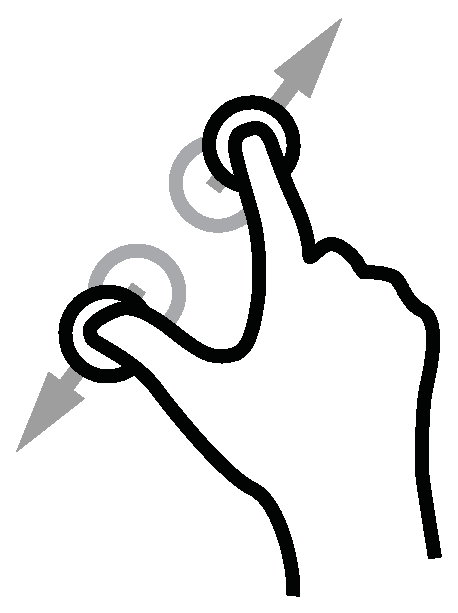
\includegraphics[width=0.2\textwidth]{two_finger_scale_gestureworks.eps}
}
\caption{Gesten}
\label{fig:gestures}
\end{figure}

\subsection{Preview}
Ein optionales Zusatzfeature ist eine Seek-Funktion mit Preview, d.h. während die Seek-Geste (s. Abbildung \ref{fig:seek}) ausgeführt wird, soll ein Vorschaubild der aktuellen Suchposition innerhalb des Streams angezeigt werden. Abbildung \ref{fig:youtube} zeigt einen ähnlichen Ansatz des YouTube-Players. Hier wird auf einer Zeitleiste beim Mouse-Over ein entsprechender Tooltip angezeigt.

\begin{figure}[H]
\centering
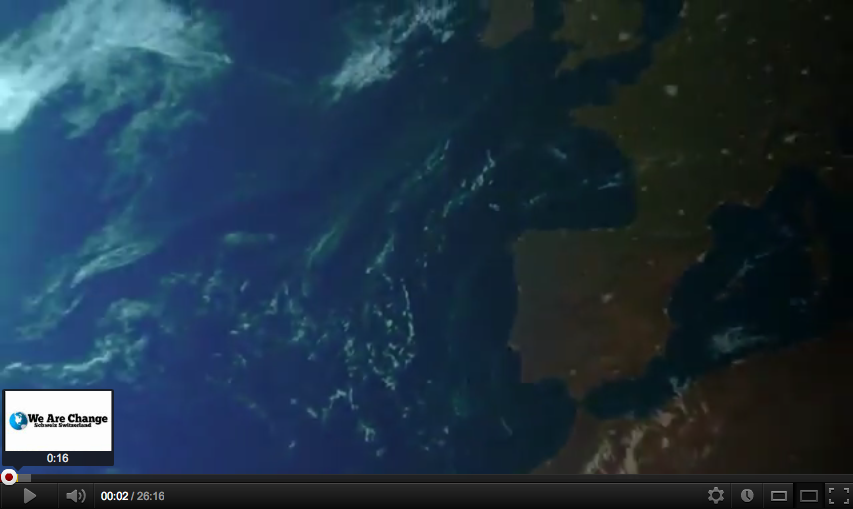
\includegraphics[width=0.75\textwidth]{youtube.png}
\caption{YouTube Preview Feature}
\label{fig:youtube}
\end{figure}

Die konkrete Darstellung muss natürlich für Smartphones separat konzipiert und entwickelt werden. Die besondere technische Herausforderung wird das Interagieren der Remote- und der Streaming-Schnittstelle sein, da die einzelnen Vorschaubilder über den Stream beschafft werden müssen.

\begin{figure}[H]
\centering

\includegraphics[width=0.35\textwidth]{vlc.png}
\end{figure}
\newpage

\subsection{Technologien}
Aus der Problemstellung wird zunächst ersichtlich, dass für die Umsetzung zwei verschiedene Komponenten betrachtet werden müssen. Dies ist einerseits die Software, die zum Abspielen und Streamen der Medieninhalte zuständig ist, sowie anderseits das mobile Endgerät, das als Fernsteuerung dienen wird. \\
Für den Mediaplayer soll der VLC Media Player von VideoLan \cite{VLC} benutzt werden. Diese Software ist sowohl kostenlos, als auch für die gängigen Betriebssysteme verfügbar. Somit kann ein weiter Einsatz gewährleistet werden. Weiterhin besitzt der VLC eine HTTP-Schnittstelle \cite{VLC:WebInterface}, über die mittels \textit{controls} (Kontrollkommandos z.B. Start/Stop) und \textit{commands} (Einstellungen z.B. Lautstärke) der Player gesteuert werden kann \cite{VLC:HowTo}. \\
Auf der Seite des mobilen Endgeräts fiel die Wahl auf die verbreitete Android-Plattform \cite{Android}. Die Entwicklung von Software für dieses System ist ohne Einschränkung der Entwicklungsumgebung möglich und die Distribution ist kostengünstiger und einfacher, als seine Konkurrenzsysteme. Den Entwicklern liegen bereits Smartphones mit verschiedenen Android-Versionen vor, um den Echtzeitbetrieb für eine breite Verteilung zu entwickeln und zu testen.

\subsection{Portierbarkeit}
Um die Ausbaufähigkeit der Anwendung sicherzustellen, wäre es wünschenswert, wenn es nur minimale Abhängigkeiten an den VLC Media Player als zu steuernde Software gibt. So wäre es in einer weiteren Ausbaustufe möglich dem Nutzer der App anzubieten diverse Video Player zu steuern, sofern sie unterstützt werden. Die Grundlage für diese Möglichkeit sollte dadurch sichergestellt werden, dass die eigentliche Kommunikation mit dem VLC Media Player innerhalb des Systems mithilfe sinnvoll definierter Schnittstellen gekapselt wird.

\newpage
\section{Projektplanung}

Für die Realisierung dieses Projektes gilt folgender Meilensteinplan:

\subsection{Version 1, \date{11.05.2012}}
\begin{itemize}
\item Evaluierung des VLC-HTTP-Schnittstellenumfangs
\item Layout aus den Vorgaben erstellen
\item Umsetzung der ersten Steuerungskomponenten
\end{itemize}

\subsection{Version 2, \date{08.06.2012}}
\begin{itemize}
\item Implementierung der weiteren Steuerungsfunktionen
\item Evaluierung der Übermittlung von Metadaten an das Mobilgerät
\item Implementierung der Previewfunktionalitäten
\end{itemize}

\subsection{Version 3, \date{03.07.2012}}
\begin{itemize}
\item Fertigstellung der Funktionalitäten
\item Qualitätssicherung
\item Installation auf mobilen Testgeräten
\end{itemize}

\section{Projektaufteilung}
Die Entwicklung des Projektes wird zu gleichen Teilen auf die Entwickler Schönborn und Feldmann getragen, wobei die Zuständigkeiten wie folgt verteilt werden:

\begin{table}[h!b!p!]
\begin{tabular*}{\textwidth}{ l l l l }
	\toprule
\textbf{Aufgabe} & \textbf{Version} & \textbf{Entwickler} \\
	\midrule
	Gestenentwicklung & 1 & Willi Schönborn  \\ 
	User Interface & 1, 2 & Willi Schönborn \\
	Gestenerkennung & 2 & Willi Schönborn \\
	VLC HTTP Interface & 1, 2 & Andreas Feldmann \\
	Remote Control Interface & 1, 2 & Andreas Feldmann \\
	Streaming & 2 & Andreas Feldmann \\
	\bottomrule
\end{tabular*}
\end{table}

\newpage

\section{Dokumentation}
\subsection{VLC mit HTTP-Interface starten}
Ab Version 2.x wurde das HTTP-Interface durch eine LUA Schnittstelle ersetzt, um die Wiedergabe scripten zu können. Das HTTP-Interface wird dabei nicht mehr standardmäßig mit geladen und ist somit auch nicht nach Programmstart verfügbar. Um das Interface für den Remotezugriff dennoch nutzen zu können,  muss das Programm mit dem Parameter \textit{--extraintf=http} gestartet werden. Dieses wird dann in der Konsolenausgabe bestätigt. \\
\begin{figure}[H]
\centering
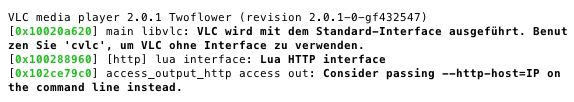
\includegraphics[width=0.75\textwidth]{cli-output.jpg}
\caption{VLC Konsolenausgabe}
\end{figure}
Hier ist gut sichtbar, dass die HTTP-Requests über das LUA-Interface geleitet werden. Die Aktivierung in den Einstellungen, wie es vor Version 2.x möglich war, existiert nicht mehr. Weiterhin können mit den Parametern  \textit{--http-host \textbf{host}} und \textit{--http-port \textbf{port}} die IP, sowie der Port angegeben werden, unter dem das Interface zu erreichen ist. Um dies zu testen kann man jetzt die Adresse \textit{http://host:port} (Standard: \textit{http:127.0.0.1:8080}) in einem Webbrowser aufrufen und erhält bei Erfolg ein HTML-Interface zur Steuerung. \\
Die einzelnen Bedienelemente senden bei Benutzung eine jQuery-Request an den VLC-Player und benutzt dabei die \textit{command:value} Syntax.
\begin{lstlisting}[caption=Play Button Command][label=code:command_button_query]
$('#buttonPlPlay').click(function(){
					sendCommand({
						'command': 'pl_play',
						'id':$('.jstree-clicked','#libraryTree').first().parents().first().attr('id').substr(5)
					})
					return false;
				});
\end{lstlisting}

\subsection{Verfügbare Kommandos}
Da die Dokumentation für die Version ab 2.x sich mit den Commands im Quelltext unterscheidet, werden die aus der Beispielanwendung extrahiert und getestet.
Die folgenden Befehle konnten gefunden werden:\\
\begin{table}
\caption{VLC Command Beschreibung}

\begin{center}
\begin{tabular}{|>{\bfseries}l|c|}
  \hline
  Command & Funktion\\
  \hline\hline
  pl\_play & Playlisteintrag abspielen \\
  pl\_stop & Wiedergabe stoppen \\
  pl\_previous & Einen Titel zurückspringen \\
  pl\_next & Zum nächsten Titel springen \\
  pl\_empty & Playlist leeren \\
  pl\_loop & Loop einschalten \\
  pl\_repeat & Playlisteintrag wiederholen \\
  pl\_random & Zufallsmodus ein/aus \\
  \hline
\end{tabular}
\label{tab:vlc_commands}
\end{center}
\end{table}

Diese Commands sind für den Betrieb des VLC essentiell und werden für die Anfangsphase der Applikationserstellung von größter Wichtigkeit sein. \\
Für die Einstellungen wie Lautstärke oder Seek kann aus dem Quelltext wenig erschlossen werden. Allein die Methoden, um die Werte zu bekommen ist zu finden, sie zu setzen nicht.

\newpage
\subsection{Architektur}
Die Applikation wurde auf den Grundlagen von Java 6 und dem Androidsystem Version 2.3 entwickelt. Die Entscheidung für diese Version wurde getroffen, da Android 2.3 für die meisten etwas älteren Geräte die momentane aktuellste Betriebssystemversion darstellt (ca. 63,6\% \cite{marktanteil-android} ) . Eine Entwicklung für Android "Ice Cream Sandwich" (Android 4.0) würde die älteren Geräte von der Benutzung ausschließen und nur ca. 11\% der Endgeräte abdecken \cite{marktanteil-android}. \\
Weiterhin wurden bei der Entwicklung die Frameworks Guava, Guice, RoboGuice, Lifegycle und Slf4j Android benutzt auf die im Folgenden eingegangen wird.
\subsubsection{Guava}
Das Guava Framefowrk von Google wurde eingesetzt, um eine Publisher-Subscriber Kommunikation, in Guava \textbf{EventBus} genannt, zwischen den Komponenten in der Applikation aufzubauen. Dieser Kommunikation wird mit Hilfe von Annotation im Code realisiert, somit müssen die Komponenten, anders als bei EventListener, nicht explizit untereinander registriert sein. Zum Vergleich ein Beispielcode mit "klassischer" Javalösung und der selbe Code mit Guava:\\
\lstset{language=Java}
\begin{lstlisting}[caption={klassische Javalösung \cite{guava-libaries} }]
    class ChangeRecorder {
     void setCustomer(Customer cust) {
       cust.addChangeListener(new ChangeListener() {
         public void customerChanged(ChangeEvent e) {
           recordChange(e.getChange());
         }
       };
     }
   }
\end{lstlisting}\newpage
\lstset{language=Java}
\begin{lstlisting}[caption={Lösung mit Guava \cite{guava-libaries}}]
    // Class is typically registered by the container.
   class EventBusChangeRecorder {
     @Subscribe public void recordCustomerChange(ChangeEvent e) {
       recordChange(e.getChange());
     }
   }
\end{lstlisting}
Durch die Verwendung der Guava Libaries wird der Code einerseits deutlich lesbarer, da die Intention des EventHandlings besser hervortritt, andererseits auch kürzer, da die anonymen Listener Implementierungen wegfallen und somit lediglich der notwendige Code für die Reaktion auf das Event implementiert werden muss.
\subsubsection{Guice, RoboGuice \& Lifegycle}
Gucie ist ein von Google entwickeltes Framework für Java, welches erlaubt, Java-Klassen mittels Dependency Injection zu konfigurieren. Die Hauptintention von Guice ist es, keine Factorymethoden mehr schreiben zu müssen, sondern die Erstellung und Bindung bestimmter Objekte durch Injections steuern zu können. Dadurch soll der Code deutlich lesbarer, einfacher zu testen und besser wiederverwendbar gestaltet werden. \\
RoboGuice wurde ebenfalls von Google entwickelt und nutzt die Vorteile und Techniken des Guice Frameworkes für Android aus. Es besticht vor allem durch den Vorteil, zum Beispiel Views und Ressourcen mittels Dependency Injection einzufügen.  Im Folgenden ist ein Beispiel zu sehen, wie der Unterschied einer herkömmlichen Android Activity und einer, die das RoboGuice Framework nutzt, aussieht:\\
\lstset{language=Java}
\begin{lstlisting}[caption={Standard Android Activity \cite{roboguice-libaries} }]
    class AndroidWay extends Activity { 
    TextView name; 
    ImageView thumbnail; 
    LocationManager loc; 
    Drawable icon; 
    String myName; 

    public void onCreate(Bundle savedInstanceState) { 
        super.onCreate(savedInstanceState); 
        setContentView(R.layout.main);
        name      = (TextView) findViewById(R.id.name); 
        thumbnail = (ImageView) findViewById(R.id.thumbnail); 
        loc       = (LocationManager) getSystemService(Activity.LOCATION_SERVICE); 
        icon      = getResources().getDrawable(R.drawable.icon); 
        myName    = getString(R.string.app_name); 
        name.setText( "Hello, " + myName ); 
    } 
} 
\end{lstlisting}
\lstset{language=Java}
\begin{lstlisting}[caption={Android Activity mit RoboGuice \cite{roboguice-libaries}}]
   class RoboWay extends RoboActivity { 
    @InjectView(R.id.name)             TextView name; 
    @InjectView(R.id.thumbnail)        ImageView thumbnail; 
    @InjectResource(R.drawable.icon)   Drawable icon; 
    @InjectResource(R.string.app_name) String myName; 
    @Inject                            LocationManager loc; 

    public void onCreate(Bundle savedInstanceState) { 
        super.onCreate(savedInstanceState); 
        setContentView(R.layout.main);
        name.setText( "Hello, " + myName ); 
    } 
} 
\end{lstlisting}
Gut zu erkennen ist, dass mit Hilfe des RoboGuice Frameworkes die Attribute im Konstruktor nicht mehr explizit gesetzt werden müssen, sondern durch Annotationen vor dem Attribut eingefügt werden.\\
Livegycle ist eine kleine Bibliothek, die für die durch Guice oder RoboJuice injizierten Objekte ein Lebenszyklusmanagement bereitstellt. Dieses Management erfolgt ebenfalls durch Annotationen und erlaubt es dem Entwicklern zu bestimmten Zeitpunkten (z.B. AfterInjection, PreDestroy, PostConstruction) das Objekt zu manipulieren oder es direkt an bestimmte Methoden zu übergeben.\cite{lifegycle-libaries}

\subsubsection{SLF4J Android}
Simple Logging Facade for Java Android ist eine umstrukturierte Variante der bekannten SLF4J Libary. welche es erlaubt zur Laufzeit den Code an vorhandene Loogingmechanismen (z.B. java.util.logging, log4j) anzubinden. Für Android wurde sie zudem mit einer simplen Weiterleitung aller Log-anfragen an den Android Logger erweitert. Der Logger wird wie in der reinen Java-Variante benutzt, lediglich das Log-Level \textbf{TRACE} heißt in Android \textbf{VERBOSE}, die anderen besitzen den gleichen Namen. \cite{sfl4j-android-libaries}
\subsection{Module}

Die \textbf{Gesture Remote} wurde bei der Konzeption in verschiedene Module aufgeteilt, um einerseits die Entwicklung parallel betreiben zu können, andererseits um die Applikation möglichst offen für Erweiterungen zu gestalten. Denkbar wären hier beispielsweise das Hinzufügen neuer Gesten oder Unterstützung anderer Mediaplayer bzw. weiterer Protokolle. 

\subsubsection{Command}
Im Commandmodul sind die einzelnen Kommandos für die Steuerung des VLC-Players hinterlegt. Da sich manche der Befehle auf den Player an sich oder auf die Steuerung der Playlist beziehen können, wurden diese Befehle auch im Code sinnvollerweise in \textit{playback} und \textit{playlist} gegliedert.
\subsubsection{Recognition}
Das Recognition Modul ist wohl das wichtigste Modul in der Applikation. Hier werden die vom Nutzer eingegebenen Gesten verarbeitet. Dabei wird für die einfache Gesten (z.B. Tap, Fling/Scroll) ein gemeinsamer Erkennungsdienst eingesetzt, für komplexe Gesten wie z.B. Pinch/Zoom wird jeweils ein eigener Dienst benutzt (z.B. PinchZoomRecognizer).
\subsubsection{Remote}
Dieses Modul deckt die Fernbedienungsfunktionen der Applikation ab. Einfach Befehle wie Play/Pause, aber auch nicht lineare Attributveränderungen, wie z.B. die prozentuale Steigerung der Lautstärke in Bezug auf die Länge der Geste sind hier untergebracht. Von hier aus werden die Kommandos, die die Gestenerkennung erfolgreich erkannt hat, an den VLC-Player als Query-Strings geschickt.
\subsubsection{Server}
Im Servermodul sind die Funktionalitäten hinterlegt, welche die Applikation mit einem laufenden VLC-Player verbindet. Die Verbindungsdaten für eine erfolgreiche Verbindung sind in einer SQLite Datenbank hinterlegt, welche sich auf jedem Android per Standard befindet. Durch diese Datenhaltung müssen keine externen Daten nachgeladen werden und der Benutzer kann auch in Netzwerken ohne Internetanschluss die Applikation benutzen.
Die Daten werden in einer einzigen Tabelle gespeichert, welche die Felder für \textit{Adresse} und \textit{Port}, sowie einen Bezeichner \textit{Name} um den Servern eine Bezeichnung zu geben und sie somit einfacher identifizieren zu können. Ein Beispiel hierfür wäre: \\
BHT-Server, 141.64.64.101:8080 (\textit{Name}, \textit{Adresse}:\textit{Port})\\

\newpage
\subsection{Installationsanleitung}
Um die Applikation auf dem Endgerät nutzen zu können sind folgende Schritte notwendig:
\begin{enumerate}
\item Den Quellcode aus dem Git Repository klonen \\git://github.com/whiskeysierra/gesture-remote.git
\item Einbinden des Projektes in eine Entwicklungsumgebung z.B. Eclipse oder IntelliJ
\item Das Projekt muss nun kompiliert werden, mit der Option es auf dem angeschlossen Mobilgerät zu deployen
\item VLC Player mit HTTP Interface starten. Der einfachste Weg ist es, den Player über die Konsole (Unix: Bash, Mac: Terminal, Windows: cmd) mit dem Parameter \textit{--extraintf=http} zu starten. Anschließend zu Testzwecken sollten mindestens 2 verschiedene Mediendateien in die Playlist eingefügt werden.
\item Auf dem Mobilgerät einen neuen Server mit der Adresse des Rechners und dem Port 8080 (Standardwerte für VLC) anlegen und verbinden
\item Auf dem Hauptview die Gestensteuerung benutzen
\end{enumerate}
\newpage

\subsection{Bedienungsanleitung}
Nach dem Starten der Applikation auf dem Mobilgerät landet man auf dem Welcomescreen der Anwendung. 
\begin{figure}[H]
\centering
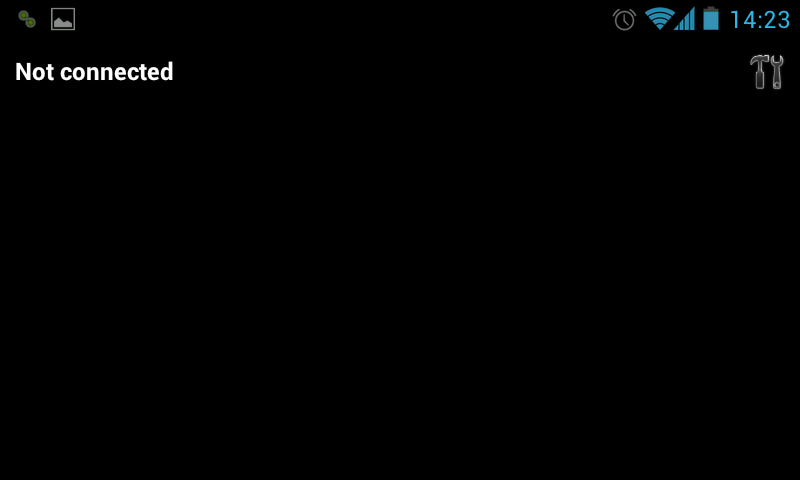
\includegraphics[width=0.75\textwidth]{Screenshot_1.png}
\caption{Startbildschirm}
\end{figure}
Anschließend kann man mit einem Tap auf das Werkzeugsymbol zu den verfügbaren Servern gelangen. Hier sind alle gespeicherten Serverdaten aufgelistet und können angewählt werden. Da bei Auslieferung der Applikation noch keine Daten hinterlegt sind, wird mit einem Tap auf das Plus Symbol in der rechten oberen Ecke die Maske für die Erstellung eines neuen Datensatzes aufgerufen.
\begin{figure}[H]
\centering
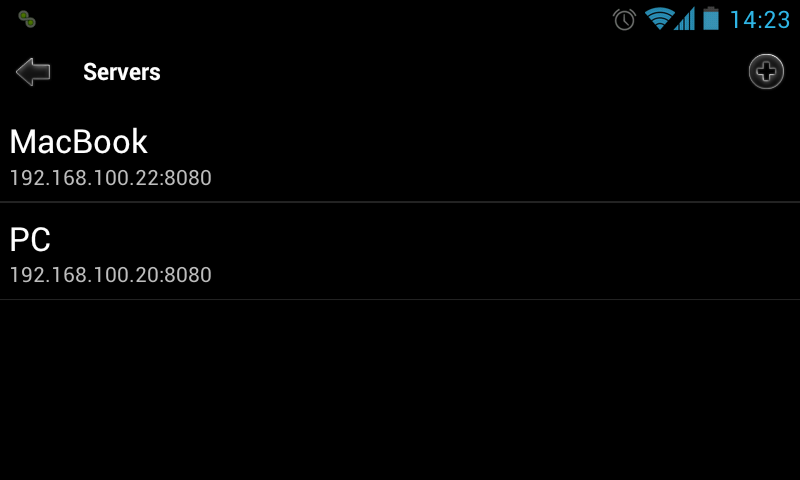
\includegraphics[width=0.75\textwidth]{Screenshot_2.png}
\caption{Servermanagement}
\end{figure}
In der Maske muss nun mindestens die Adresse oder der Hostname, sowie der Port eingegeben werden, unter dem der Rechner erreichbar ist, auf dem der VLC Player läuft. Es wird geraten, einen bezeichnenden Namen zu vergeben, um die Daten auseinanderhalten zu können.
\begin{figure}[H]
\centering
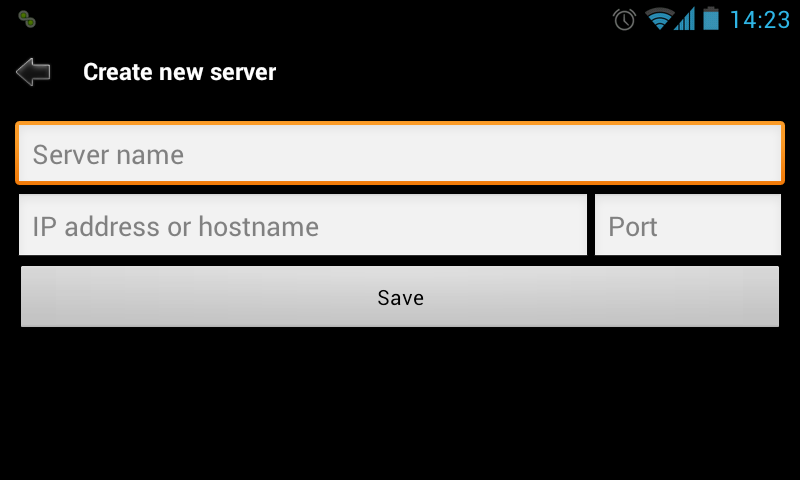
\includegraphics[width=0.75\textwidth]{Screenshot_3.png}
\caption{Neuen Server anlegen}
Als Beispiel wurde hier der Server mit dem Namen PC unter der Adresse 192.168.100.20:8080 angelegt.
\begin{figure}[H]
\centering
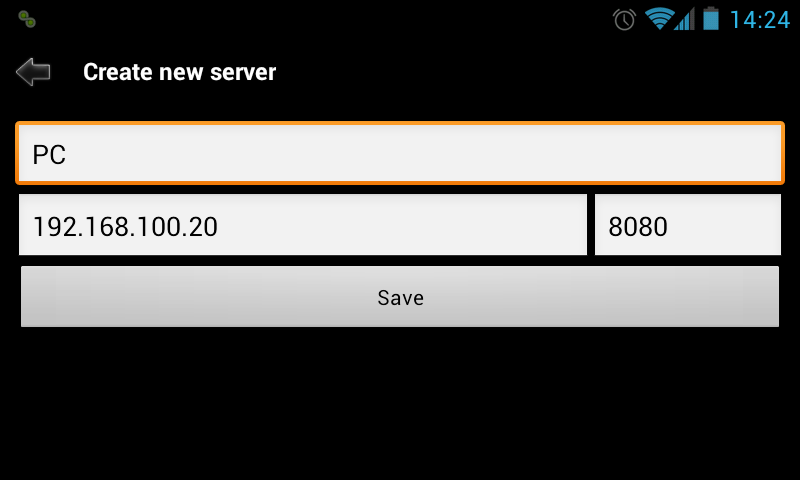
\includegraphics[width=0.75\textwidth]{Screenshot_5.png}
\caption{Neuer Datensatz}
\end{figure}
\end{figure}
Mittels eines Tap auf den Datensatz öffnet sich ein PopUp Menü, in dem man entweder den Datensatz löschen, editieren oder mittels der Daten eine Verbindung zum VLC herstellen kann.
\begin{figure}[H]
\centering
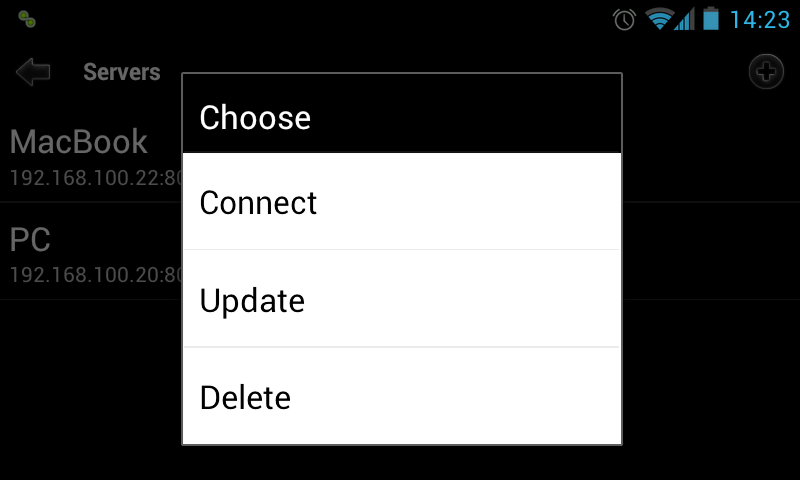
\includegraphics[width=0.75\textwidth]{Screenshot_4.png}
\caption{PopUp Menü}
\end{figure}
Nach der Auswahl des Menüpunktes "Choose" versucht sich die Applikation mit dem Server als Remote zu verbinden. Bei Erfolg wird auf dem Startbildschirm die Nachricht \textit{Connected to \textbf{ServerName}} angezeigt. Nun kann der Player mit den Gesten gesteuert werden
\begin{figure}[H]
\centering
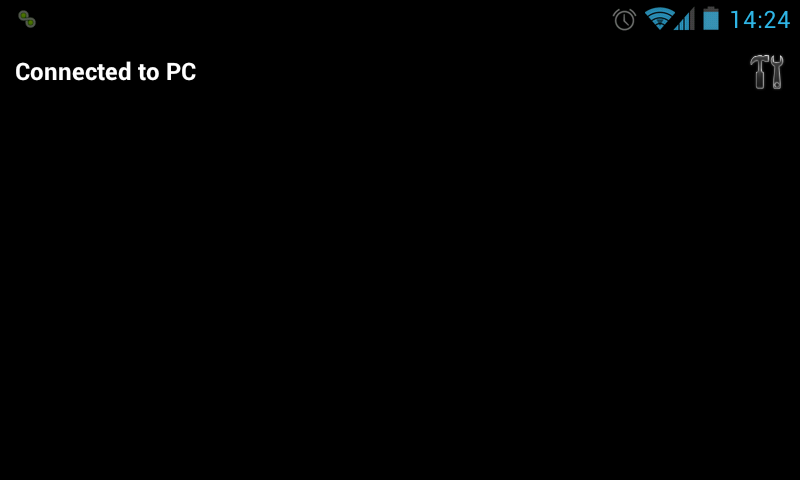
\includegraphics[width=0.75\textwidth]{Screenshot_6.png}
\caption{Verbindung hergestellt}
\end{figure}
Die Abbildungen \ref{fig:play} und \ref{fig:pause} zeigen die Ausgabe nach der Tap Geste, also dem einmaligen Berühren des Bedienfeldes. Diese Geste schaltet vom Abspielmodus in den Pausemodus und umgekehrt.  
\begin{figure}[H]
\centering
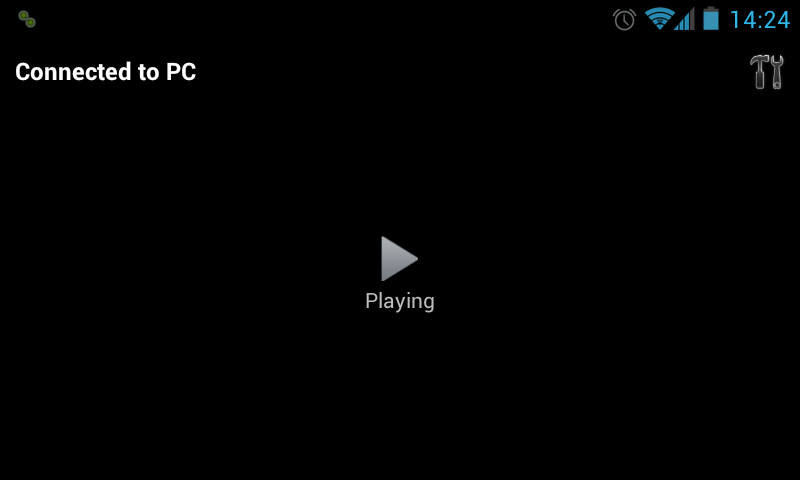
\includegraphics[width=0.75\textwidth]{Screenshot_7.png}
\caption{Play}
\label{fig:play}
\end{figure}
\begin{figure}[H]
\centering
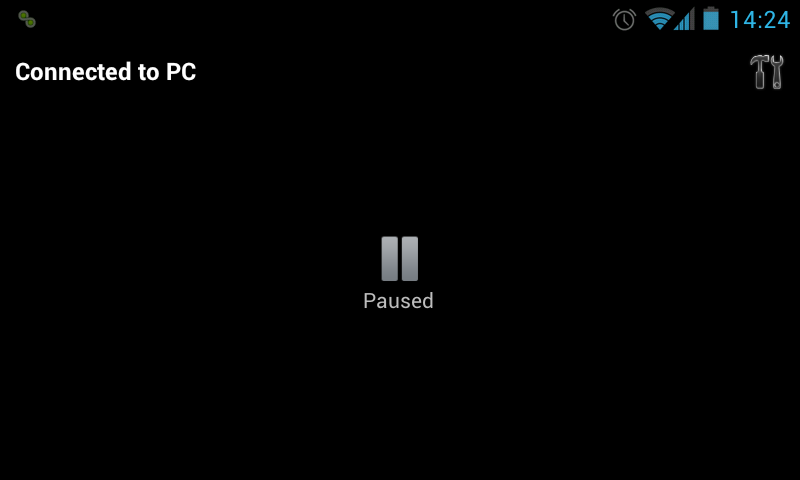
\includegraphics[width=0.75\textwidth]{Screenshot_8.png}
\caption{Pause}
\label{fig:pause}
\end{figure}
An der rechte Seite der Applikation befindet sich das Bedienfeld für die Lautstärkeregelung. Mittels der Drag-Geste (kontinuierliches Zeichnen) wird die Lautstärke Prozentual in die Gestenrichtung angepasst. Damit soll eine Schiebereglerregelung emuliert werden, wie sie z.B. beim Mischpult noch genutzt wird. 
\begin{figure}[H]
\centering
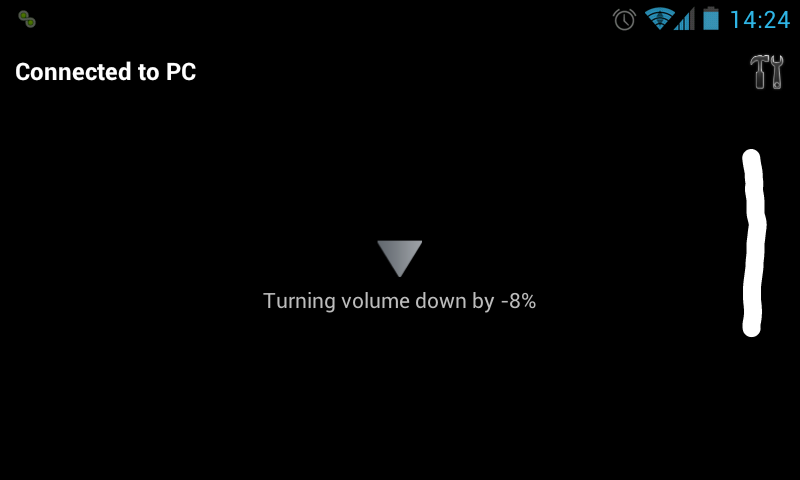
\includegraphics[width=0.75\textwidth]{Screenshot_9.png}
\caption{Lautstärkeregelung}
\end{figure}
Die Drag-Geste wird außerdem am unteren Rand des Bildschirmes erkannt, allerdings nur, wenn sie hier horizontal ausgeführt wird. Durch diese Geste wird der Player angewiesen vor- bzw. zurückzuspulen. Durch einen Tap wird der Spulvorgang unterbrochen und der Player wird wieder in den Abspielmodus versetzt.
\begin{figure}[H]
\centering
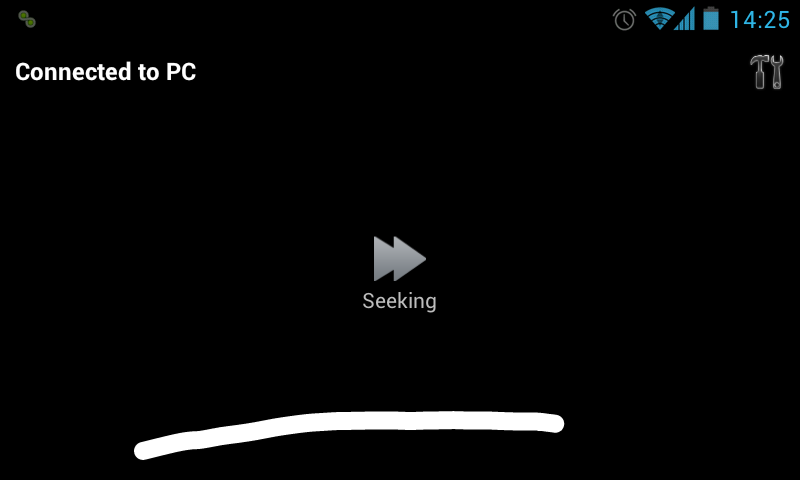
\includegraphics[width=0.75\textwidth]{Screenshot_10.png}
\caption{Seek-Funktion}
\end{figure}
Da man nicht immer vor- bzw. zurückspulen will, sondern ganze Titel oder Kapitelmarken überspringen will, wurde auf der Hauptview die Swipe-Geste eingefügt. sie erlaubt es, zur nächsten Markierung in die Richtung der Geste zu springen. So kann man sich durch eine Playlist, aber auch durch z.B. DVD-Kapitel navigieren.
\begin{figure}[H]
\centering
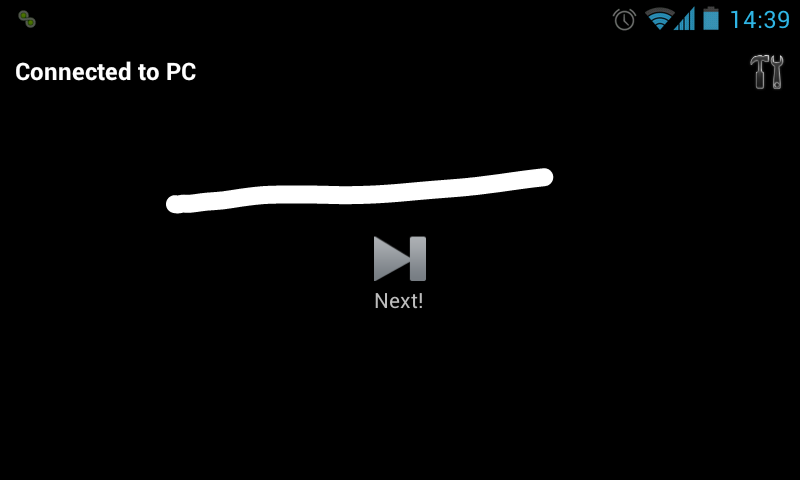
\includegraphics[width=0.75\textwidth]{Screenshot_11.png}
\caption{Nächster/Vorheriger Titel}
\end{figure}

\section{Fazit}
Bei der Entwicklung der Gestenerkennung traten 2 große Probleme auf. Einerseits musste die Benutzung einer selbst entwickelten Geste, bei der man kontinuierlich einen Kreis zeichnet, fallen gelassen werden. Die Gestenerkennung arbeitet hier nicht schrittweise, sondern versucht erst nach der Beendigung des Zeichenvorganges die Geste anhand der aufgenommenen Punkte zu erkennen. Einen einfachen Kreis zu zeichnen und diesen  erkennen lassen stellt kein Problem dar, das fortlaufende Zeichnen, um z.B. die Spulgeschwindigkeit einzustellen, allerdings schon, da hier erst nach dem letzten Punkt die Geste erkannt wird und diese ist dann kein Kreis mehr, sondern eine unregelmäßige Spirale mit sich überlagernden Pfaden. Somit musste diese Geste aus der Applikation entfallen. Dafür wurde der horizontale und vertikale Drag für das Spulen bzw. die Lautstärke eingeführt. Dies führte allerdings zur zweiten Problematik der Gestenerkennung. Die Drag Geste ist der Swipe Geste sehr ähnlich und könnte einerseits zu Verwirrungen des Benutzers, aber auch zu Problemen der Unterscheidung bei der Erkennung führen. Daher wurde entschieden, den Drag Gesten bestimmte Bereiche zuzuweisen, in denen sie ausgeführt werden können. In den anderen Bereich sind dann nur nie Swipe-Gesten gültig. Um die Anwendung trotzdem intuitiv bedienbar zu gestalten, wurden diese Bereiche so gewählt, dass sie den bekannten Programmen oder Geräten ähneln. So wurde, wie in den meisten Videoplayern üblich, der untere Bereich dafür genutzt um vor- oder zurückzuspulen. Für die Lautstärke wurde der rechte seitliche Bereich gewählt, um so einen Schieberegler zu emulieren, wie er bei Stereoanlagen oder Mischpulten üblich ist, da sich wie bereits beschrieben, die Drehregelung nicht umsetzen lies.\\
Ein geplantes Playlistmanagment auf dem Mobilgerät wurde verworfen, da der Bildschirm zu klein ist, um vernünftige Drag\&Drop Funktionalität über Listen mit mehr als 5 Einträgen gewährleisten zu können. Auch das hinzufügen von Titeln kann über das Mobilgerät nicht erfolgen, da die Dialoge vom Betriebssystem des Rechners auf das Mobilgerät übertragen werden müssen und die Handlings darauf wieder zurück an den Rechner. Dies ist in der momentanen Entwicklungsstufe nicht möglich.\\
Aus Zeitgründen wurden die Previewfunktionalitäten von Videodaten nicht in das Projekt integriert. Einerseits muss der VLC dafür in 2 Modi laufen, einem fernsteuerbaren und einem streambaren und dies funktionierte in den Testfällen nur selten. Außerdem war die korrekte Übertragung und Darstellung auf das Mobilgerät problematisch. \\
Über den Zeitpunkt dieser Vorlesung hinweg, kann das Projekt dennoch erweitert werden und bietet ein guten Ansatzpunkt zur Weiterentwicklung und Überlegungen, wie man die Problematiken lösen kann, sodass die Features doch noch genutzt werden können. Eine weitere Möglichkeit wäre der Ansatz einer Schnittstellenentwicklung für weitere Medienplayer, womit man ein breiteres Spektrum der Anwendungsunterstützung anbieten könnte. Alles in allem bietet die dieses abgeschlossene Projekt vielfältige Möglichkeiten der Weiterentwicklung und kann auch produktiv bereits genutzt werden. 
\newpage
\addcontentsline{toc}{section}{Literatur}
\nocite{*}
\printbibliography

\newpage
\addcontentsline{toc}{section}{Abbildungsverzeichnis}
\listoffigures

\addcontentsline{toc}{section}{Tabellenverzeichnis}
\listoftables

\addcontentsline{toc}{section}{Quellcodeverzeichnis}
\renewcommand{\lstlistlistingname}{Quellcodeverzeichnis}
\lstlistoflistings

\end{document}

